\section{Introdução} \label{introduction}

% O texto da introdução deve: • ser construído de acordo com as partes constituintes do texto (fazendo um brevíssimo resumo de cada uma delas)
% Quanto aos seus elementos, uma introdução deve:
% a) apresentar a ideia central do trabalho, ou seja, o tema da pesquisa que foi realizada e da qual o trabalho é o resultado;
% b) deixar clara a finalidade do trabalho, ou seja, os objetivos da pesquisa;

Gestão de laboratórios é extremamente necessária no mundo tecnológico em que vivemos hoje. Aumento de eficiência, automação de processos, gestão de tempo e funcionários são algumas das funcionalidades que são procuradas atualmente em diversos laboratórios \cite{sun2021laboratory}. Para esse tipo de gestão, é necessário algum meio de formalizar fluxos de trabalhos para que sejam de fácil entendimento e reproduzíveis. Para isso, temos os BPMs.

BPMs (Business Process Models) são modelos de fluxos de trabalho utilizados para definir como processos serão realizados, definindo objetivos dentro de uma organização \cite{Alves2014}. Eles podem ser utilizados para abstrair fluxos de trabalho existentes e criar novos fluxos com maior facilidade, podendo ser construídos seguindo a notação de BPMs, a BPMN (Business Process Model and Notation) \cite{Dijkman2008}.

BPMs podem ser utilizados para gerar modelos de negócio para diversos tipos de fluxos de trabalho (exemplo de um método ágil implementada em BPM na figura \ref{fig:bpm}), como telemedicina e bioinformática, sendo implementado em hospitais, laboratórios e empresas privadas. Os BPMs facilitam na gestão, automação e acompanhamento de um fluxo de trabalho.

\begin{figure}
    \centering
    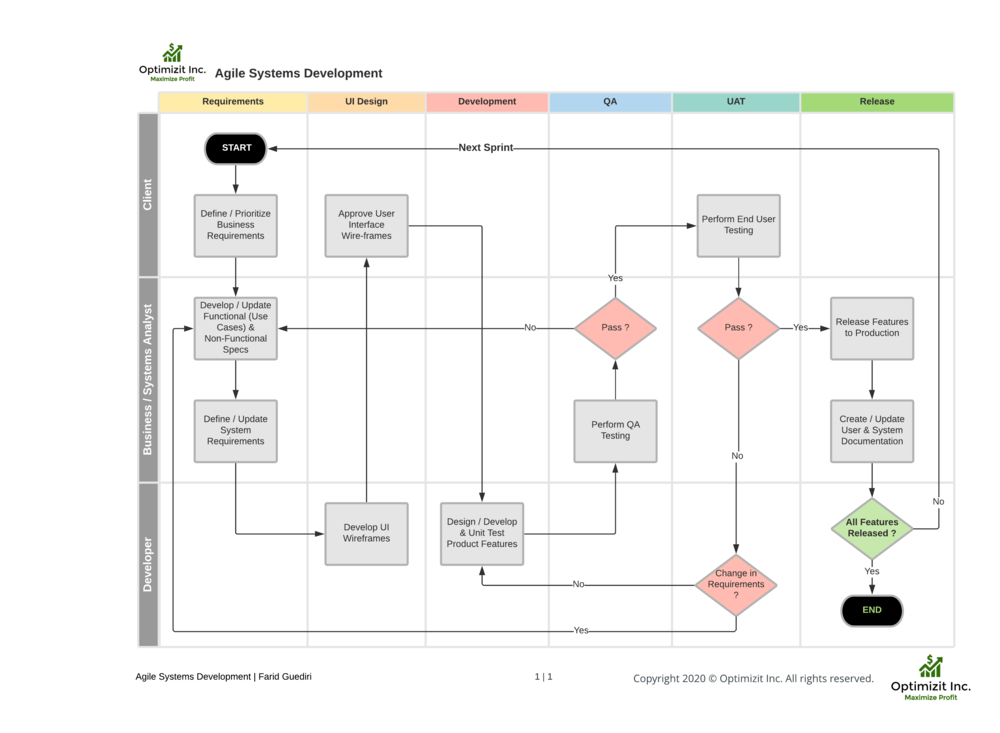
\includegraphics[width=1\textwidth]{imgs/BPM/sprint as bpm.png}
    \caption{Exemplos de um método ágil modelado como um BPM}
    \label{fig:bpm}
\end{figure}

Com isso, surgem os LIMS (Laboratory Information Management Systems) que, utilizando BPMs, conseguem organizar o fluxo de trabalho dentro de um laboratório para maior automação de processos e aumento da eficiência de cada etapa dentro de um determinado escopo \cite{Key2011}. Os LIMS nada mais são que softwares criados especificamente ou genericamente para um fluxo de trabalho específico.

A utilização de um LIMS traz grandes vantagens para laboratórios que o utilizam, como a automação de processos e coleta e armazenamento de dados \cite{Key2011}. Os LIMS usam de BPMs para abstrair atividades (uma ação dentro do BPM) que podem ser repetidas ou não, como em experimentos que devem ser refeitos ou atendimento a pacientes. 

Um BPM pode conter várias atividades que podem ou não depender uma das outras. No caso de um laboratório, realizar um experimento seria considerado uma atividade, calibração das máquinas seria outra atividade, obtenção de produtos também se transforma em outra atividade.

Para um fluxo de trabalho muito grande, temos uma profundidade grande nas atividades (como veremos na figura \ref{fig:centrareEstrutura}), ou seja, existe um ramo de atividades uma seguida da outra em sequência. Nós chamaremos isso de profundidade de atividades dentro do fluxo.

Caso uma atividade esteja muito profunda no ciclo do BPM (para chegar até ele, deve ser passado por muitas atividades anteriores), temos o problema de acesso desta atividade pelo usuário no LIMS, ou seja, muita informação (que podem ser desnecessárias) é mostrada ao usuário até que ele chegue à atividade esperada.

A proposta desse trabalho é alterar a visualização do BPM dentro do LIMS, dando mais facilidade para que o usuário acesse, preencha e complete suas tarefas com maior praticidade e agilidade dentro do espaço de trabalho, sem a necessidade de passar pelas atividades anteriores à desejada.

Também existe um problema de falta de compartilhamento de atividades entre BPMs, o que deixa o fluxo de trabalhos laboratoriais travado para um workflow em específico, já que uma atividade pode necessitar de informações de outras atividades (como um paciente que pode ter informações importantes junto a outros familiares também pacientes). Assim, o trabalho de implementar o compartilhamento de tais atividades entre diferentes fluxos de trabalho para que os dados sejam compartilhados entre setores ou até mesmo entre laboratórios está sendo feito, permitindo a unificação de BPMs com atividades em comum.

Testamos a implementação já existente da troca de ordem de atividades nos seguintes workflows: CENTRARE, um fluxo de trabalho para o Centro de Tratamento e Reabilitação de Fissura Labiopalatal e Deformidade Craniofacial do hospital da baleia, em belo horizonte, e o workflow BPL (Boas Práticas de Laboratório), que tem como finalidade registrar informações sobre os procedimentos usados no laboratório.